	
	Validaremos ahora el comportamiento de nuestro modelo con datos reales con secuencias discretas distribuidas no uniformemente.
	
	
	
	\begin{figure}[h] 
		\centering
				\resizebox{0.6\textwidth}{!}{% <------ Don't forget this %
			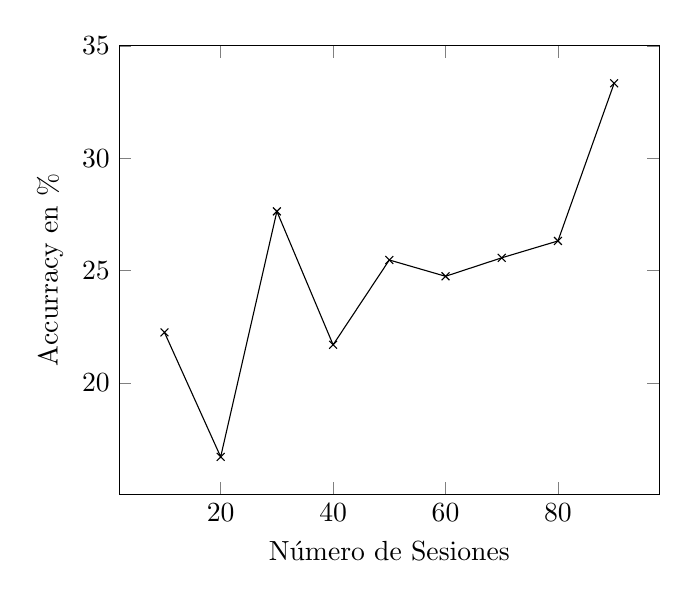
\begin{tikzpicture}
			\begin{axis}[
			xlabel= Número de Sesiones,
			ylabel=Accurracy en \% ]
			\addplot[color=black,mark=x] coordinates {
				(10, 22.2471910112359)
				(20, 16.7088607594936)
				(30, 27.6328502415459)
				(40, 21.6949152542372)
				(50, 25.469387755102)
				(60, 24.7435897435897)
				(70, 25.5665024630541)
				(80, 26.3157894736842)
				(90, 33.3333333333333)
			};
			\end{axis}
			\end{tikzpicture}
		}
		\caption{Experimento con secuencias de largo variable}
		\label{fig:experimento2}
	\end{figure}
	

	\begin{table}[h]
		\centering
		\label{tabla-exp-1}
		\begin{tabular}{ccccc}
			\textbf{pruebas}     & \textbf{entrenamiento} & \textbf{accuracy}    & \textbf{nodos}       & \textbf{niveles}     \\
			10                   & 90                     & 0,222471910112359    & 10                   & 5                    \\
			20                   & 80                     & 0,167088607594936    & 10                   & 5                    \\
			30                   & 70                     & 0,27632850241546     & 10                   & 5                    \\
			40                   & 60                     & 0,21694915254237     & 10                   & 5                    \\
			50                   & 50                     & 0,25469387755102     & 10                   & 5                    \\
			60                   & 40                     & 0,24743589743590   	 & 10                   & 5                    \\
			70                   & 30                     & 0,255665024630541    & 10                   & 5                    \\
			80                   & 20                     & 0,263157894736842    & 10                   & 5                    \\
			90                   & 10                     & 0,333333333333333    & 10                   & 5                    \\
			&                        &                      &                      &                      \\
			\multicolumn{1}{l}{} & \multicolumn{1}{l}{}   & \multicolumn{1}{l}{} & \multicolumn{1}{l}{} & \multicolumn{1}{l}{}
		\end{tabular}
		\caption{ Resumen de datos experimento 1}
	\end{table}



	\begin{table}[h] 	\label{tabl-exp-1-frec}
		\centering
		\resizebox{0.9\textwidth}{!}{% <------ Don't forget this %
	
		\begin{tabular}{lccccccccccccccccc}
			\textbf{símbolo}    & A  & B  & C  & D  & E & F  & G  & H  & I  & J  & K & L  & M  & N  & O & P & Q \\
			\textbf{frecuencia} & 64 & 19 & 18 & 29 & 4 & 36 & 20 & 65 & 20 & 11 & 4 & 15 & 42 & 31 & 2 & 0 & 0
		\end{tabular}
		
	}
		\caption{Tabla de frecuencia experimento 1}
	\end{table}


			
	En este caso si existe una menor redundancia a diferencia del experimento \ref{exp1} lo que produce que el modelo $M$ tenga un bajo rendimiento, aún así dada sigue siendo en el mejor de los casos seis veces mejor que la probabilidad aleatoria de predecir. En este experimento usamos un $|\sigma| =15$, por ende tenemos que dado nuestro modelo,
	\begin{equation}\label{expResult2}
		M( x | \mbox{90\% train}  ) = 33 \% \geq M( x | \mbox{random}  ) = 6.66 ,\% 
	\end{equation} como hemos visto en el experimento \ref{exp1} nuestro modelo sigue siendo válido en un escenario en que los datos se dispersan considerablemente. 
	Adicionalmente en este tipo de caso existe un comportamiento de nuestro modelo en el cual hace el mejor esfuerzo por mantener la \emph{compresibilidad} de los datos mayor o igual a la \emph{predictibilidad} del mismo, peor al tener mayor dispersión la altura para una cantidad similar de sesiones en \ref{exp1} sigue siendo $5$. Pero la cantidad de nodos sufre un gran incremento, podemos verlo en \ref{fig:exp-largo-variable-inf}
	
	
	
	\begin{figure}[h] 
		\centering
		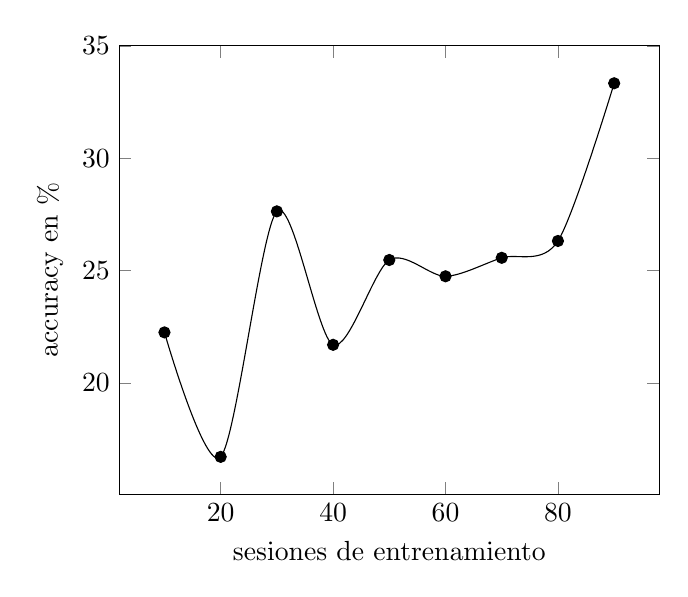
\begin{tikzpicture}
		\begin{axis}[
		xlabel=$\mbox{sesiones de entrenamiento}$,
		ylabel=$\mbox{accuracy en \%}$]
		\addplot[smooth,mark=*,black] plot coordinates {
			(10, 22.2471910112359)
			(20, 16.7088607594936)
			(30, 27.6328502415459)
			(40, 21.6949152542372)
			(50, 25.469387755102)
			(60, 24.7435897435897)
			(70, 25.5665024630541)
			(80, 26.3157894736842)
			(90, 33.3333333333333)
		};
		\end{axis}
		\end{tikzpicture}	
		
		\caption{Experimento con secuencias de largo variable inferiores y 100 sesiones}
		\label{fig:exp-largo-variable-inf}
	\end{figure}
	
	
	



	Acorde al gráfico \ref{fig:exp-largo-variable-inf} podemos señalar que al haber un incremento en la dispersión de datos y menor redundancia, el crecimiento de nuestro árbol será horizontal, ya que para tanto como hemos en este experimento y en (\label{expResult2}), la altura del nodo no tiene una relación directa a la redundancia ó dispersión, pero si a la cantidad de sesiones evaluadas. 
	
	Además, al mayor esfuerzo que hace el predictor por lograr mejores resultados se construyen mas nodos, por lo que el modelo LDC, deja de comprimir por satisfacer las condiciones de predictibilidad necesarias para seguir siendo válido.

	
	Iteramos una nueva evaluación con las mismas condiciones pero subiendo el volumen de datos de 100 a 1000. Con este buscaremos ver encontrar el mismo comportamiento a un mayor nivel de datos.
	


	
	
	\begin{figure}[t] 
		\centering
		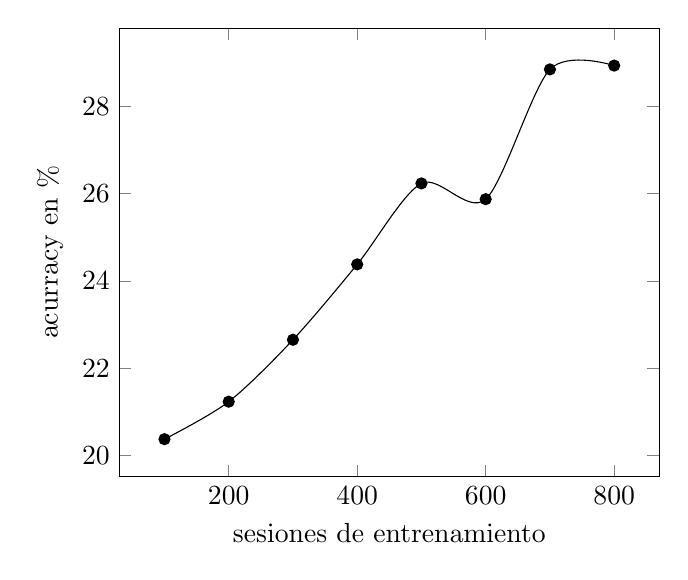
\begin{tikzpicture}
		\begin{axis}[
		xlabel=$\mbox{sesiones de entrenamiento}$,
		ylabel=$\mbox{acurracy en \%}$]
		\addplot[smooth,mark=*,black] plot coordinates {
			(100,  20.3715239154616)
			(200,  21.2302878598247)
			(300,  22.6490224129709)
			(400,  24.3752086811352)
			(500,  26.2308617234469)
			(600,  25.8692564745196)
			(700,  28.8423315814619)
			(800,  28.929431438127)
		};
		\end{axis}
		\end{tikzpicture}
		\caption{Experimento con secuencias de largo variable inferiore y 1000 sesiones}
		\label{fig:sim}
	\end{figure}
	
	El modelo sigue siendo válido al ir aumentando el volumen de datos bajo las mismas circunstancias. Incluso para ambos experimentos anteriores podemos sacar la relación que nuestro modelo posee una tasa de error de $\pm4\%$ al aumentar $100$ veces con respecto a la primera iteración de este escenario cuando se usa la  mayor cantidad de sesiones de entrenamiento posible.


	Otra particularidad que ha demostrado el modelo gracias a las propiedades de compresibilidad expuestas por  \emph{Lempel} \& \emph{Ziv}\cite{ZivLempel1977} es la minimización de niveles requeridos aún cuando la cantidad de nodos va creciendo.
	
	
	
	
	\begin{figure}[h] 
		\centering
			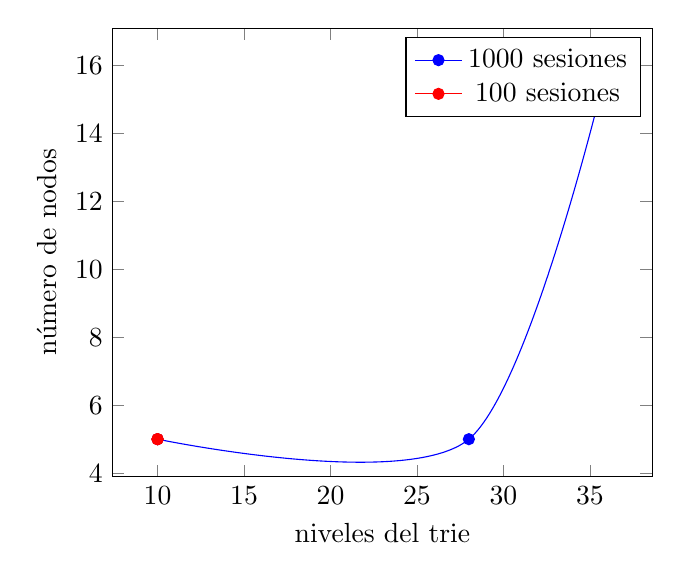
\begin{tikzpicture}
			\begin{axis}[
			xlabel=$\mbox{niveles del trie}$,
			ylabel=$\mbox{número de nodos}$]
			\addplot[smooth,mark=*,blue] plot coordinates {
				( 10 , 5 )
				( 28 , 5)
				( 36 , 16)
			};
			\addlegendentry{ 1000 sesiones }
			\addplot[smooth,mark=*,red] plot coordinates {
				( 10,5 )
				( 10,5 )
				( 10,5 )
			};
			\addlegendentry{ 100 sesiones }
			\end{axis}
			\end{tikzpicture}
		\caption{Gráfico comparativo para mismos niveles distinta cantidad de nodos.}
		\label{fig:sim}
	\end{figure}
	
	


	Como podemos ver en el comportamiento de inicio del modelo el criterio de partida en el escenario descrito es compartido por ambos experimentos.

	También dado a que no es uno de los escenarios más favorables para nuestro modelo predictivo, podríamos tener un diferencial en los tiempos de construcción del \emph{trie} respecto a la cantidad de nodos necesarios para el entrenamiento, 

	\begin{figure}[h] 
	\centering
	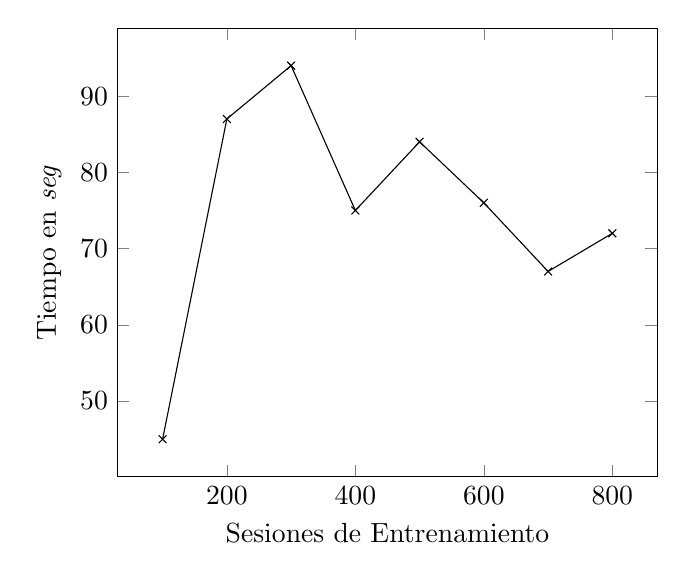
\begin{tikzpicture}
	\begin{axis}[
		xlabel= Sesiones de Entrenamiento ,
		ylabel= Tiempo en \emph{seg} ]
	\addplot[color=black,mark=x] coordinates {
			(100, 45 )
			(200, 87 )
			(300, 94 )
			(400, 75 )
			(500, 84 )
			(600, 76 )
			(700, 67)
			(800, 72 )
	};
	\end{axis}
	\end{tikzpicture}
		\caption{Gráfico de tiempo de construcción vs sesiones de entrenamiento}
	  \label{fig:sim}
	 \end{figure}	
	
	Como podemos ver en el gráfico anterior podemos buscar un dataset óptimo el cual puede encontrarse dentro del intervalo $ [ 300,400 ]$ sesiones de usuario, equivalente a la mejores resultados de \emph{Accurracy} y menor cantidad de secuencias de entrenamiento.